\clearpage
\subsectionold{MSVC: x86 + \olly}

Proviamo ad hackerare il nostro programma in \olly, forzandolo a pensare che \scanf funzioni sempre senza errori.
Quando l'indirizzo di una variabile locale e' passato a \scanf, la variabile inizialmente contiene un valore random inutile, in questo caso \TT{0x6E494714}:

\begin{figure}[H]
\centering
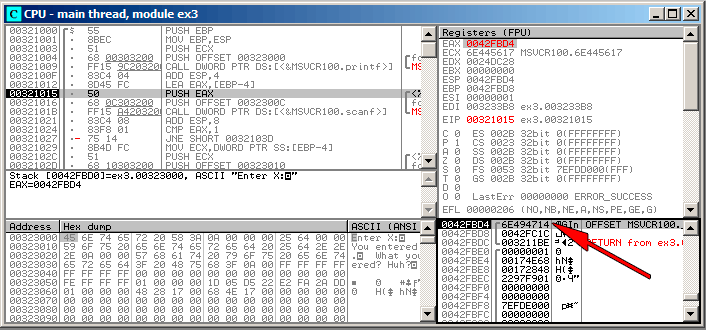
\includegraphics[scale=\FigScale]{patterns/04_scanf/3_checking_retval/olly_1.png}
\caption{\olly: passing variable address into \scanf}
\label{fig:scanf_ex3_olly_1}
\end{figure}

\clearpage
Quando \scanf viene eseguita, immettiamo nella console qualcosa di diverso da un numero, come \q{asdasd}.
\scanf finisce con 0 in \EAX, indicante che un errore si e' verificato:

\begin{figure}[H]
\centering
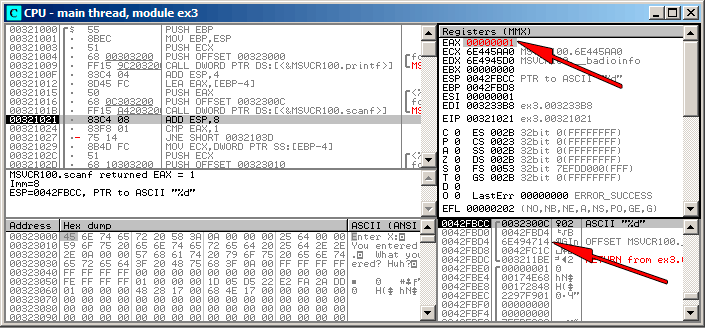
\includegraphics[scale=\FigScale]{patterns/04_scanf/3_checking_retval/olly_2.png}
\caption{\olly: \scanf returning error}
\label{fig:scanf_ex3_olly_2}
\end{figure}

Possiamo anche controllare la variabile locale nello stack e notare che non e' stata modificata.
Infatti cosa avrebbe potuto scrivere \scanf in essa? Non ha fatto niente oltre che restituire zero. 


Proviamo ad \q{hackerare} il nostro programma.
Click destro su \EAX, 
Tra le opzioni vediamo \q{Set to 1}.
Esattamente cio' che ci serve.

Adesso abbiamo 1 in \EAX, il controllo successivo sta per essere eseguito come previsto,
e \printf stampera' il valore della variabile nello stack.

Quando avviamo il programma (F9) vediamo il seguente output nella finestra della console:

\begin{figure}[H]
\centering
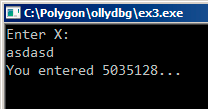
\includegraphics[scale=\FigScale]{patterns/04_scanf/3_checking_retval/olly_3.png}
\caption{console window}
\end{figure}

1850296084 e' infatti la rappresentazione decimale del numero nello stack (\TT{0x6E494714})!
